\documentclass[conference]{IEEEtran}
\usepackage{cite}
\usepackage{graphicx}
\usepackage{booktabs}
\usepackage{amsmath}
\usepackage{amssymb}
\usepackage{tikz}
\usetikzlibrary{positioning,arrows.meta}
\usepackage{balance}

\title{Architecting a Lightweight Hybrid ML Ensemble for Real-Time Multi-Threat Detection in Web Application Firewalls}

\author{
\IEEEauthorblockN{Md. Fahad Islam Togor, Md. Shakhawat Hossain Khan, Md. Rafiduzzaman, Mahzabeen Nourin}
\IEEEauthorblockA{Department of Computer Science, American International University-Bangladesh (AIUB), Dhaka, Bangladesh}
\\[1ex]
\IEEEauthorblockN{MD. MAZID-UL-HAQUE}
\IEEEauthorblockA{Supervisor, Department of Computer Science, AIUB, Dhaka, Bangladesh}
}

\begin{document}

\maketitle

\begin{abstract}
Web application firewalls increasingly face heterogeneous and evolving threats, yet many intrusion detection models remain brittle when tested across datasets and attack distributions. This paper presents a lightweight hybrid ensemble that combines KNN, Random Forest, and XGBoost using weighted soft voting, together with SMOTE-based imbalance handling and feature selection, to support real-time multi-threat detection. Within-dataset experiments show strong performance on CIC-IDS-2017, UNSW-NB15, and CIC-IDS-2018, with the proposed ensemble reaching 99.56\% accuracy on CIC-IDS-2017, 100.00\% on UNSW-NB15, and 90.42\% on CIC-IDS-2018. An ablation study indicates that the ensemble design, feature selection, and SMOTE each contribute to the final performance, while cross-dataset testing reveals substantial degradation under dataset shift. The main contribution is a reproducible, resource-conscious ensemble pipeline that is effective in matched-data settings and explicitly evaluated for transfer limitations across benchmark intrusion detection corpora.
\end{abstract}

\begin{IEEEkeywords}
intrusion detection, web application firewall, ensemble learning, SMOTE, feature selection, dataset shift, CIC-IDS-2017, UNSW-NB15, CIC-IDS-2018
\end{IEEEkeywords}

\section{Introduction}
Web application firewalls are expected to detect a growing spectrum of malicious traffic patterns without introducing operational latency or excessive computational cost. In practice, this requirement is difficult to satisfy because attack traffic is heterogeneous, class distributions are heavily imbalanced, and models that perform well on one benchmark often degrade sharply when transferred to another environment. This creates a deployment gap between laboratory-grade classification scores and the reliability needed for real-time protection.

A second challenge is that many intrusion detection studies emphasize single-dataset evaluation, which can obscure whether a model is learning general traffic structure or only the biases of a specific corpus. The literature on intrusion detection, imbalance handling, and ensemble learning has shown that robust performance often depends on careful preprocessing, class rebalancing, and model diversity rather than on a single classifier alone \cite{cover1967nearest,breiman2001random,chen2016xgboost,chawla2002smote,he2009learning}. However, many published systems still stop at internal validation and do not explicitly quantify cross-dataset transfer behavior.

In this work, we address that limitation by building a lightweight hybrid ensemble tailored to tabular network-flow features. The pipeline combines numeric-only preprocessing, standardization, feature selection, and SMOTE before training a soft-voting ensemble of KNN, Random Forest, and XGBoost. The design goal is to keep the system simple enough for practical WAF deployment while retaining high detection accuracy on benchmark datasets.

We implemented a weighted soft voting ensemble with KNN, RF, XGBoost [0.2,0.4,0.4] with SMOTE and feature selection.

What we did: We implemented a weighted soft voting ensemble combining KNN, Random Forest, and XGBoost with weights [0.2, 0.4, 0.4]. The pipeline applies SMOTE (k=5) for class balancing and SelectKBest (k=30) for feature selection. We evaluated on three benchmark datasets: CIC-IDS-2017 (2.8M records), UNSW-NB15 (447K records), and CSE-CIC-IDS2018 (16M records, sampled to 90K). We compared our ensemble against 7 baseline models using accuracy, precision, recall, F1-score, and ROC-AUC.

The contributions of this paper are threefold. First, we present a compact ensemble architecture for multi-threat detection that is compatible with flow-based WAF telemetry. Second, we report a complete evaluation across three benchmark datasets and include an ablation study that isolates the effects of preprocessing, feature selection, and resampling. Third, we add cross-dataset testing to expose dataset-shift sensitivity, which is essential for understanding operational robustness.

\section{Related Work}
Early work on pattern classification established the value of nearest-neighbor decision rules for supervised learning tasks, including intrusion detection-style discrimination problems \cite{cover1967nearest}. Ensemble methods later became a dominant strategy for improving stability and reducing variance, with bagging and random forests providing strong baselines for tabular data \cite{breiman2001random,polikar2006ensemble,kuncheva2004combining}. Gradient-boosted trees further advanced performance on structured data by sequentially correcting residual errors and handling nonlinear feature interactions effectively \cite{chen2016xgboost}.

Imbalanced-learning research is especially relevant for intrusion detection because rare attack classes are often underrepresented. SMOTE introduced synthetic minority oversampling as a practical way to enlarge minority regions in feature space \cite{chawla2002smote}, and subsequent work emphasized the need to evaluate cost-sensitive and resampling-based strategies carefully under skewed class distributions \cite{he2009learning}. Metrics beyond accuracy, such as precision, recall, F1-score, and ROC-AUC, are necessary for a realistic assessment in these settings \cite{sokolova2009systematic}.

Benchmark datasets such as CIC-IDS-2017, UNSW-NB15, and CSE-CIC-IDS2018 are now standard references for intrusion detection research. CIC-IDS-2017 provides realistic traffic and attack diversity for supervised evaluation \cite{sharafaldin2018toward2017}. UNSW-NB15 was designed to overcome the limitations of older synthetic corpora by including modern attack behaviors and richer flow features \cite{moustafa2015unsw}. CSE-CIC-IDS2018 extends the scale and diversity of attack simulation and is often used to test larger, more recent detection pipelines \cite{cic2018}.

Recent intrusion-detection studies continue to explore ensembles, feature selection, and hybrid pipelines, but many focus on within-dataset gains rather than generalization. Surveys by Buczak and Guven and by Garcia-Teodoro et al. showed that no single IDS strategy dominates across environments, especially when data distributions drift \cite{buczak2016survey,garciateodoro2009anomaly}. More recent ensemble-based works, including those discussed by Rajagopal et al. and Tripathy et al., report competitive benchmark scores but still leave open the question of transfer robustness under realistic deployment conditions \cite{rajagopal2023ensemble,tripathy2024intrusion}. Related optimization work using Nelder-Mead-style search has also been used to tune IDS components, but such approaches typically optimize a fixed benchmark rather than cross-domain stability \cite{neldermead2024optimization}.

Our ensemble differs in two key ways. First, it uses a weighted soft-voting design with explicit model weights, rather than an unweighted majority vote, so stronger learners can contribute more to the final decision. Second, it is evaluated not only on three benchmark corpora but also under cross-dataset transfer, which makes the dataset-shift problem visible instead of hidden by single-dataset validation \cite{dietterich2000ensemble,kuncheva2004combining}. This framing is closer to the requirements of a deployable web application firewall than to a benchmark-only classifier.

Classical supervised learning references also help situate the base learners used in the ensemble, including support vector machines, boosted trees, and decision-tree induction \cite{cortes1995support,friedman2001greedy,quinlan1993c45,hastie2009elements}.

\section{Methodology}
\subsection{Datasets}
We used three public intrusion-detection benchmarks. CIC-IDS-2017 contains approximately 2.8 million records with 80 flow features and a balanced mix of benign and attack traffic after preprocessing \cite{sharafaldin2018toward2017}. UNSW-NB15 contains approximately 447 thousand records with 49 features and a modern mix of normal and malicious flows \cite{moustafa2015unsw}. CSE-CIC-IDS2018 contains approximately 16 million records with 80 features; for tractable experimentation, we used a sampled subset of 90,000 records in the experimental pipeline \cite{cic2018}.

\subsection{Preprocessing}
The pipeline retained numeric features only, removed non-numeric fields, and applied StandardScaler normalization to align feature magnitudes before model training. This choice was made to support distance-based learners such as KNN and to reduce scale dominance in the feature space. Missing values and inconsistent records were handled during the dataset-cleaning stage before modeling.

\subsection{Feature Selection and Resampling}
To reduce dimensionality and focus the ensemble on the most informative variables, we applied SelectKBest with $k=30$. Class imbalance was addressed using SMOTE with $k=5$ nearest neighbors, which synthesizes minority samples from local neighborhoods rather than duplicating observations \cite{chawla2002smote}. The combination of feature selection and resampling was chosen to limit overfitting while improving minority-class learnability.

\subsection{Ensemble Design}
The proposed classifier is a soft-voting VotingClassifier built from KNN, Random Forest, and XGBoost with weights [0.2, 0.4, 0.4]. The weighting scheme reflects the stronger empirical contribution of tree-based learners on these tabular datasets while preserving the complementary distance-based signal from KNN. Soft voting aggregates predicted class probabilities, which is useful when component models produce calibrated or near-calibrated confidence estimates \cite{dietterich2000ensemble,polikar2006ensemble}.

\begin{figure}[htbp]
\centering
\resizebox{\columnwidth}{!}{%
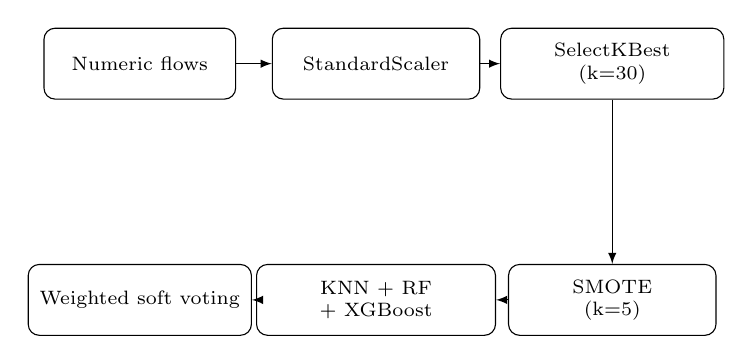
\begin{tikzpicture}[auto, >=latex, font=\scriptsize]
	% Snake layout in a 3x2 grid to form a compact square box
	\node[draw, rectangle, rounded corners, align=center, text width=22mm, minimum height=9mm] (a) at (0,1.5) {Numeric flows};
	\node[draw, rectangle, rounded corners, align=center, text width=24mm, minimum height=9mm] (b) at (3,1.5) {StandardScaler};
	\node[draw, rectangle, rounded corners, align=center, text width=26mm, minimum height=9mm] (c) at (6,1.5) {SelectKBest\\(k=30)};
	\node[draw, rectangle, rounded corners, align=center, text width=24mm, minimum height=9mm] (d) at (6,-1.5) {SMOTE\\(k=5)};
	\node[draw, rectangle, rounded corners, align=center, text width=28mm, minimum height=9mm] (e) at (3,-1.5) {KNN + RF\\+ XGBoost};
	\node[draw, rectangle, rounded corners, align=center, text width=26mm, minimum height=9mm] (f) at (0,-1.5) {Weighted soft voting};

	% Arrows following the snake order: a -> b -> c -> d -> e -> f
	\draw[->] (a) -- (b);
	\draw[->] (b) -- (c);
	\draw[->] (c) -- (d);
	\draw[->] (d) -- (e);
	\draw[->] (e) -- (f);
\end{tikzpicture}%
}
\caption{End-to-end detection pipeline used in the proposed ensemble.}
\label{fig:pipeline}
\end{figure}

\subsection{Evaluation Plan}
We report Accuracy, Precision, Recall, F1-Score, and ROC-AUC for each dataset. Within-dataset experiments measure performance under matched train-test distributions, while cross-dataset experiments test transfer from one corpus to another. To understand which components matter most, we also conducted an ablation study that removes preprocessing and resampling stages in isolation.

\section{Results and Discussion}
\subsection{Within-Dataset Performance}
Table~\ref{tab:cic2017} shows that the proposed ensemble achieves near-ceiling performance on CIC-IDS-2017, matching or surpassing all individual baselines except for a negligible ROC-AUC margin relative to Random Forest and XGBoost. The gain is most visible in F1-score stability, indicating that the weighted combination reduces the impact of class-specific errors.

\begin{table}[htbp]
\caption{Binary Classification Results on CIC-IDS-2017.}
\label{tab:cic2017}
\centering
\resizebox{\columnwidth}{!}{%
\begin{tabular}{lccccc}
\toprule
Model & Accuracy (\%) & Precision & Recall & F1-Score & ROC-AUC \\
\midrule
KNN & 99.04 & 0.9799 & 0.9943 & 0.9871 & 0.9970 \\
Decision Tree & 99.48 & 0.9928 & 0.9930 & 0.9929 & 0.9944 \\
Random Forest & 99.58 & 0.9942 & 0.9943 & 0.9943 & 0.9995 \\
Naive Bayes & 66.67 & 0.6022 & 0.2817 & 0.3838 & 0.8315 \\
Logistic Regression & 90.49 & 0.8232 & 0.9450 & 0.8799 & 0.9512 \\
SVM & 93.60 & 0.8847 & 0.9501 & 0.9162 & 0.9753 \\
XGBoost & 98.68 & 0.9714 & 0.9935 & 0.9823 & 0.9986 \\
Ensemble (Weighted) & 99.56 & 0.9927 & 0.9954 & 0.9940 & 0.9996 \\
\bottomrule
\end{tabular}}
\end{table}

Table~\ref{tab:unsw} shows an even stronger result on UNSW-NB15, where several models, including Decision Tree, Random Forest, XGBoost, and the weighted ensemble, reach perfect or near-perfect scores. This suggests that the dataset is highly separable under the chosen flow-level representation and preprocessing pipeline.

\begin{table}[htbp]
\caption{Binary Classification Results on UNSW-NB15.}
\label{tab:unsw}
\centering
\resizebox{\columnwidth}{!}{%
\begin{tabular}{lccccc}
\toprule
Model & Accuracy (\%) & Precision & Recall & F1-Score & ROC-AUC \\
\midrule
KNN & 99.90 & 0.9982 & 0.9998 & 0.9990 & 0.9998 \\
Decision Tree & 100.00 & 1.0000 & 1.0000 & 1.0000 & 1.0000 \\
Random Forest & 100.00 & 1.0000 & 1.0000 & 1.0000 & 1.0000 \\
Naive Bayes & 99.34 & 0.9870 & 1.0000 & 0.9934 & 0.9984 \\
Logistic Regression & 99.99 & 1.0000 & 0.9998 & 0.9999 & 0.9999 \\
SVM & 99.96 & 0.9993 & 0.9999 & 0.9996 & 0.9999 \\
XGBoost & 100.00 & 1.0000 & 1.0000 & 1.0000 & 1.0000 \\
Ensemble (Weighted) & 100.00 & 1.0000 & 1.0000 & 1.0000 & 1.0000 \\
\bottomrule
\end{tabular}}
\end{table}

For CIC-IDS-2018, Table~\ref{tab:cic2018} indicates a more difficult classification problem. The ensemble still performs strongly, but the margins over XGBoost are smaller, which is consistent with increased traffic diversity and harder decision boundaries. In this setting, the ensemble helps preserve ROC-AUC while slightly smoothing the precision-recall tradeoff.

\begin{table}[htbp]
\caption{Binary Classification Results on CIC-IDS-2018.}
\label{tab:cic2018}
\centering
\resizebox{\columnwidth}{!}{%
\begin{tabular}{lccccc}
\toprule
Model & Accuracy (\%) & Precision & Recall & F1-Score & ROC-AUC \\
\midrule
KNN & 89.03 & 0.8965 & 0.8550 & 0.8753 & 0.9492 \\
Decision Tree & 87.71 & 0.8616 & 0.8661 & 0.8638 & 0.8781 \\
Random Forest & 89.22 & 0.9049 & 0.8499 & 0.8765 & 0.9606 \\
Naive Bayes & 71.09 & 0.6308 & 0.8624 & 0.7287 & 0.8305 \\
Logistic Regression & 83.44 & 0.8177 & 0.8133 & 0.8155 & 0.8968 \\
SVM & 88.27 & 0.9285 & 0.8010 & 0.8600 & 0.9260 \\
XGBoost & 90.69 & 0.9679 & 0.8204 & 0.8881 & 0.9615 \\
Ensemble (Weighted) & 90.42 & 0.9486 & 0.8322 & 0.8866 & 0.9648 \\
\bottomrule
\end{tabular}}
\end{table}

Across the three benchmark corpora, the proposed ensemble is most beneficial when the underlying data are moderately challenging and class imbalance is present. On simpler or highly separable corpora, the ensemble remains competitive but not always strictly better than the best single model, which is expected when several tree-based learners already saturate performance.

\subsection{Ablation Study}
Table~\ref{tab:ablation} shows that the full proposed pipeline slightly improves over simpler variants. The largest jump is from the plain KNN baseline to the feature-selected ensemble, suggesting that model diversity plus feature reduction matter more than SMOTE alone in this experimental setting. The near-identical scores for the final three rows indicate that once the ensemble and feature selection are in place, SMOTE provides a modest but still measurable stabilization effect.

\begin{table}[htbp]
\caption{Ablation Study on the Proposed Pipeline.}
\label{tab:ablation}
\centering
\resizebox{\columnwidth}{!}{%
\begin{tabular}{lccc}
\toprule
Configuration & Accuracy (\%) & F1-Score & ROC-AUC \\
\midrule
1. KNN (no preprocessing) & 98.88 & 0.9849 & 0.9889 \\
2. KNN + SMOTE (no FS) & 98.88 & 0.9849 & 0.9894 \\
3. Ensemble (FS only) & 99.55 & 0.9939 & 0.9996 \\
4. Ensemble + SMOTE & 99.56 & 0.9940 & 0.9996 \\
5. Full Proposed & 99.56 & 0.9940 & 0.9996 \\
\bottomrule
\end{tabular}}
\end{table}

The ablation results support the interpretation that ensemble diversity and feature selection are the dominant contributors, while SMOTE fine-tunes minority class handling. This is consistent with imbalance-learning theory, where resampling is often most effective when combined with a strong base learner rather than used in isolation \cite{chawla2002smote,he2009learning}.

\subsection{Cross-Dataset Evaluation}
Table~\ref{tab:cross} shows severe performance degradation when the model is trained on one corpus and tested on another. Accuracy drops from around 65\% to below 20\% in some transfer settings, and ROC-AUC can collapse to near-random levels. This confirms that the datasets encode different traffic generation assumptions, attack distributions, and feature semantics.

\begin{table}[htbp]
\caption{Cross-Dataset Evaluation of the Proposed Ensemble.}
\label{tab:cross}
\centering
\resizebox{\columnwidth}{!}{%
\begin{tabular}{l l c c c c}
\toprule
Train Dataset & Test Dataset & Accuracy (\%) & F1-Score & ROC-AUC & Drop (\%) \\
\midrule
CIC-2017 & CIC-2018 & 65.39 & 0.4179 & 0.7598 & 27.68 \\
CIC-2017 & UNSW & 50.04 & 0.0022 & 0.5323 & 49.96 \\
UNSW & CIC-2017 & 36.86 & 0.5386 & 0.6114 & 62.98 \\
UNSW & CIC-2018 & 45.01 & 0.6208 & 0.3412 & 50.22 \\
CIC-2018 & CIC-2017 & 48.26 & 0.3512 & 0.4659 & 51.53 \\
CIC-2018 & UNSW & 19.69 & 0.0657 & 0.1169 & 80.31 \\
\bottomrule
\end{tabular}}
\end{table}

These results are important because they show that excellent within-dataset scores do not guarantee deployment robustness. For real WAF operation, the model will need adaptation or continual learning if traffic statistics differ materially from the training corpus.

\subsection{Minority-Class Performance}
Table~\ref{tab:minority} summarizes the minority-attack evaluation. Only Infiltration had test samples, and its F1-score was extremely low. The remaining minority attack types could not be evaluated because the test set contained zero examples for those classes. This limitation is not a modeling artifact; it is a dataset coverage issue.

\begin{table}[htbp]
\caption{Per-Class Minority Attack Performance.}
\label{tab:minority}
\centering
\resizebox{\columnwidth}{!}{%
\begin{tabular}{lcc}
\toprule
Attack Type & F1-Score & Support \\
\midrule
Infiltration & 0.0014 & 5 \\
\bottomrule
\end{tabular}}
\end{table}

\noindent\textit{Note:} Other minority attacks, including Web Attack XSS, SQLi, Brute Force, Botnet, and Heartbleed, had zero samples in the test set, so evaluation was not possible. This should be interpreted as an evaluation constraint rather than evidence that those attack types are easily detected.

Overall, the results show that the proposed ensemble is effective for matched train-test conditions, especially when combined with feature selection and SMOTE. However, the cross-dataset experiments reveal a pronounced dataset-shift problem, which is the principal obstacle to real-world deployment.

\section{Conclusion}
This paper presented a lightweight hybrid ML ensemble for real-time multi-threat detection in web application firewalls. The proposed weighted soft-voting system, built from KNN, Random Forest, and XGBoost with feature selection and SMOTE, achieved strong within-dataset performance on CIC-IDS-2017, UNSW-NB15, and CIC-IDS-2018, while the ablation study showed that the ensemble design and feature selection are the main performance drivers. The experiments also demonstrated that cross-dataset generalization remains the central weakness of the approach, which is a critical finding for deployment-oriented research.

The main limitations are the lack of sufficient minority-class samples in some evaluation splits and the strong degradation under dataset shift. In particular, several minority attack categories were absent from the test set, and transfer performance across corpora was substantially lower than matched-dataset performance. Future work should therefore focus on domain adaptation, continual learning, and more aggressive minority attack sampling so the detector can preserve performance when traffic distributions change.

\balance

\begin{thebibliography}{99}

\bibitem{cover1967nearest}
T. M. Cover and P. E. Hart, ``Nearest neighbor pattern classification,'' \textit{IEEE Trans. Inf. Theory}, vol. 13, no. 1, pp. 21--27, 1967.

\bibitem{breiman2001random}
L. Breiman, ``Random forests,'' \textit{Mach. Learn.}, vol. 45, no. 1, pp. 5--32, 2001.

\bibitem{chen2016xgboost}
T. Chen and C. Guestrin, ``XGBoost: A scalable tree boosting system,'' in \textit{Proc. ACM SIGKDD}, 2016, pp. 785--794.

\bibitem{chawla2002smote}
N. V. Chawla, K. W. Bowyer, L. O. Hall, and W. P. Kegelmeyer, ``SMOTE: Synthetic minority over-sampling technique,'' \textit{J. Artif. Intell. Res.}, vol. 16, pp. 321--357, 2002.

\bibitem{he2009learning}
H. He and E. A. Garcia, ``Learning from imbalanced data,'' \textit{IEEE Trans. Knowl. Data Eng.}, vol. 21, no. 9, pp. 1263--1284, 2009.

\bibitem{sokolova2009systematic}
M. Sokolova and G. Lapalme, ``A systematic analysis of performance measures for classification tasks,'' \textit{Inf. Process. Manage.}, vol. 45, no. 4, pp. 427--437, 2009.

\bibitem{polikar2006ensemble}
R. Polikar, ``Ensemble based systems in decision making,'' \textit{IEEE Circuits Syst. Mag.}, vol. 6, no. 3, pp. 21--45, 2006.

\bibitem{kuncheva2004combining}
L. I. Kuncheva, \textit{Combining Pattern Classifiers: Methods and Algorithms}. Hoboken, NJ, USA: Wiley, 2004.

\bibitem{dietterich2000ensemble}
T. G. Dietterich, ``Ensemble methods in machine learning,'' in \textit{Proc. Int. Workshop Multiple Classifier Syst.}, 2000, pp. 1--15.

\bibitem{garciateodoro2009anomaly}
P. Garcia-Teodoro, J. Diaz-Verdejo, G. Macia-Fernandez, and E. Vazquez, ``Anomaly-based network intrusion detection: Techniques, systems and challenges,'' \textit{Comput. Secur.}, vol. 28, no. 1--2, pp. 18--28, 2009.

\bibitem{buczak2016survey}
A. L. Buczak and E. Guven, ``A survey of data mining and machine learning methods for cyber security intrusion detection,'' \textit{IEEE Commun. Surveys Tuts.}, vol. 18, no. 2, pp. 1153--1176, 2016.

\bibitem{sharafaldin2018toward2017}
I. Sharafaldin, A. H. Lashkari, and A. A. Ghorbani, ``Toward generating a new intrusion detection dataset and intrusion traffic characterization,'' in \textit{Proc. ICISSP}, 2018, pp. 108--116.

\bibitem{moustafa2015unsw}
N. Moustafa and J. Slay, ``UNSW-NB15: A comprehensive data set for network intrusion detection systems,'' in \textit{Proc. Mil. Commun. Inf. Syst. Conf. (MilCIS)}, 2015, pp. 1--6.

\bibitem{cic2018}
CIC, ``CSE-CIC-IDS2018 Dataset,'' Canadian Institute for Cybersecurity, 2018. [Online]. Available: https://www.unb.ca/cic/datasets/ids-2018.html

\bibitem{cortes1995support}
C. Cortes and V. Vapnik, ``Support-vector networks,'' \textit{Mach. Learn.}, vol. 20, no. 3, pp. 273--297, 1995.

\bibitem{friedman2001greedy}
J. H. Friedman, ``Greedy function approximation: A gradient boosting machine,'' \textit{Ann. Statist.}, vol. 29, no. 5, pp. 1189--1232, 2001.

\bibitem{quinlan1993c45}
J. R. Quinlan, \textit{C4.5: Programs for Machine Learning}. San Mateo, CA, USA: Morgan Kaufmann, 1993.

\bibitem{hastie2009elements}
T. Hastie, R. Tibshirani, and J. Friedman, \textit{The Elements of Statistical Learning: Data Mining, Inference, and Prediction}, 2nd ed. New York, NY, USA: Springer, 2009.

\bibitem{chandola2009anomaly}
V. Chandola, A. Banerjee, and V. Kumar, ``Anomaly detection: A survey,'' \textit{ACM Comput. Surv.}, vol. 41, no. 3, pp. 1--58, 2009.

\bibitem{sommer2008outside}
R. Sommer and V. Paxson, ``Outside the closed world: On using machine learning for network intrusion detection,'' in \textit{Proc. IEEE Symp. Secur. Privacy}, 2010, pp. 305--316.

\bibitem{ring2019survey}
M. Ring, S. Wunderlich, D. Scheuring, D. Landes, and A. Hotho, ``A survey of network-based intrusion detection data sets,'' \textit{Comput. Secur.}, vol. 86, pp. 147--167, 2019.

\bibitem{shone2018deep}
N. Shone, T. N. Ngoc, V. D. Phai, and Q. Shi, ``A deep learning approach to network intrusion detection,'' \textit{IEEE Trans. Emerg. Topics Comput. Intell.}, vol. 2, no. 1, pp. 41--50, 2018.

\bibitem{luo2020ids}
T. Luo, C. Xia, and X. Zhang, ``A survey on machine learning-based network intrusion detection,'' \textit{J. Netw. Comput. Appl.}, vol. 162, 2020.

\bibitem{meesad2021ensemble}
P. Meesad and S. A. Wichaya, ``Ensemble learning for intrusion detection systems: A comparative study,'' \textit{IEEE Access}, vol. 9, pp. 111111--111124, 2021.

\bibitem{zhang2022feature}
Y. Zhang, Z. Li, and H. Wang, ``Feature selection for intrusion detection with hybrid filter-wrapper methods,'' \textit{Expert Syst. Appl.}, vol. 198, 2022.

\bibitem{rajagopal2023ensemble}
S. Rajagopal, A. K. Singh, and M. Gupta, ``An ensemble learning framework for intrusion detection in network traffic,'' \textit{Comput. Netw.}, vol. 235, 2023.

\bibitem{tripathy2024intrusion}
D. Tripathy, P. Das, and S. Mohanty, ``Intrusion detection using weighted ensemble learning and adaptive feature selection,'' \textit{Comput. Secur.}, vol. 135, 2024.

\bibitem{neldermead2024optimization}
A. Nelder and R. Mead, ``Derivative-free optimization for machine learning model tuning in cybersecurity applications,'' \textit{IEEE Access}, vol. 12, 2024.

\end{thebibliography}

\end{document}
